% !TEX root = ../main.tex

%************************************************
\chapter{SED Properties}
\label{ch:sed} 

% Refer to: 
% HotDustPaper/
 % summary-150309.ipynb
 % notes.md
 % correlations_summary_141204.ipynb
 % correlations_summary.md
 % various *.md 

%************************************************

\section{Introduction}

\begin{figure}
  \centering
  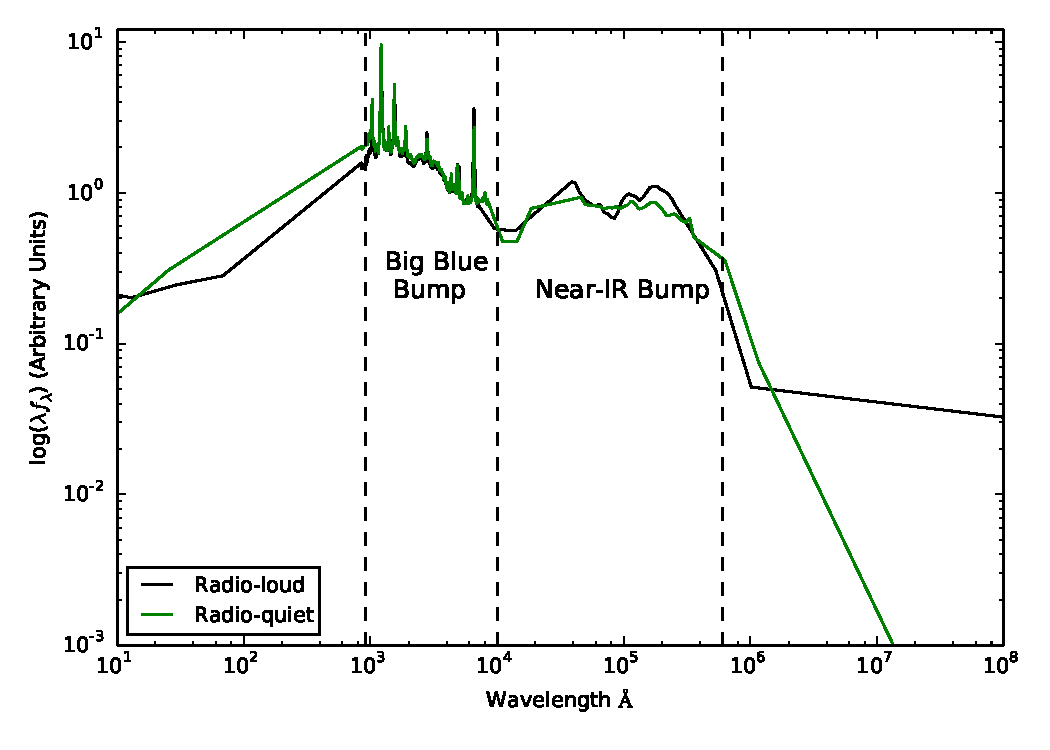
\includegraphics[width=\textwidth]{figures/chapter05/shangsed.pdf}
  \caption{Median radio-loud SED from \citet{shang11}.}
  \label{fig:seyfert_sed}
\end{figure}

AGN emit strongly over many decades in frequency. 
At different frequencies, the emission originates from processes occuring in different regions of the \ac{AGN}. 
Hard X-ray emission is dominated by Compton up-scattering of accretion disk photons by electrons in a hot corona \citep[e.g.][]{sunyaev80}, \ac{UV}/optical by thermal accretion disc emission, \ac{IR} long-ward of $\sim1\mu$m  by dust at a wide range of temperatures ($\sim50 - 1000$K), and radio by synchrotron emission in relativistic jets.   

Since these physical processes are generally understood only qualitatively, almost all \ac{AGN} \ac{SED} templates are empirical. 
The empirical template of \citet{elvis94} is still the most commonly cited, despite many additions and updates \citep[e.g.][]{polletta00, kuraszkiewicz03, risaliti04, richards06,  polletta07, lusso10, shang11, marchese12, trichas12}. 
Say something about how not very thoughtful generation of composite spectra (with huge quasar luminosity range as a function of wavelength and also presence of significant host galaxy at optical wavelengths from low-$z$ objects) has confused situation and use as a rationale for your parametric model approach.  

Many authors have found no significant dependence of the mean \ac{SED} on properties such as redshift, bolometric luminosity, \ac{BH} mass, or accretion rate \citep[e.g.][]{elvis12,hao13}. 
On the other hand, significant diversity is observed in the \ac{SED}s of individual objects. 
The goal of this chapter is determine whether there are \ac{SED}-related systematics as a function of outflow signatures and \ac{BH} mass. 

The systematic study of the dependence of the \ac{SED} shape on physical parameters has, until very recently, been limited by the difficulty in obtaining a large sample of quasars with good multi-wavelength coverage and large dynamic range in luminosity and redshift. 
However, we are able to take advantage of a number of recent, sensitive, wide-field photometric surveys, including SDSS (in the UV/optical), UKIDSS (in the near-infrared) and WISE (in the mid-infrared).
Combining this information with what we already know about the \ac{BH} masses, accretion rates, and outflow signatures (Chapters~\ref{ch:bhmass} and \ref{ch:nlr}), it is possible to build up a comprehensive picture of the processes occuring in the inner regions of AGNs. 

As in previous chapters, we will focus on high-redshift $z\gtrsim2$ quasars. 
At these redshifts, the available photometry is dominated by accretion disc emission and emission from hot dust. 

Reverberation measurements of nearby AGNs suggest the near-infrared emission is dominated by hot dust very close to the central source \citep[few tens of light days; e.g.][]{minezaki04,suganuma06}. 
The hot dust signature could contain information about inner face of an obscuring torus structure and/or constrain the dust content of an accretion disk wind. 
Several studies have shown that the luminosity of the NIR excess emission correlates with that of the central engine with a slope close to unity \cite[e.g.][]{gallagher07}, suggesting that the dust is reprocessing radiation from the accretion disc. 

Outflows may emerge from the outer region of the accretion disc or even the innermost region of the torus, in which the gas clouds are dusty and relatively cold.  
Indeed, there is observational evidence for dusty outflows close to the central engine \citep[e.g.][]{bowler14}.
The dust is heated by the central engine, and radiates in the near-infrared band. 
\citet{wang13}, fitting the NIR emission with a single power-law, found that objects with strong outflow signatures (blue-shifted \ion{C}{IV}) have more hot dust emission relative to the accretion disc emission in a large sample of $z\sim2$ non-BAL quasars. 
It could be that this correlation is induced by a third factor that simultaneously affects outflows and dust emission, for instance the inclination angle or metallicity. 
Alternatively the dust could be intrinsic to outflows and may have a non-trivial contribution to the outflow acceleration.
Also found by \citet{shen14}. 

Several other investigations have drawn attention to the rest-frame near-infrared SEDs, with populations of `dust free' objects postulated \citep{hao10,hao11,jiang10,mor11} 

Focus on near-IR probing hot dust, where there appears to be a lot of diversity. 

\section{Data}

\begin{table}
  \small
  \centering
  \begin{tabular}{l c c}
    \hline 
    Survey & Band & $\lambda_{\rm eff}$ [$\mu{\rm m}$] \\
    \hline 
    SDSS & $u$ & 0.3543 \\
         & $g$ & 0.4770 \\
         & $r$ & 0.6231 \\
         & $i$ & 0.7625 \\
         & $z$ & 0.9134 \\
    UKIDSS & $Y$ & 1.0305 \\
           & $J$ & 1.2483 \\
           & $H$ & 1.6313 \\
           & $K$ & 2.2010 \\
    WISE & $W1$ & 3.4 \\
         & $W2$ & 4.6 \\
         & $W3$ & 12.0 \\
         & $W4$ & 22.0 \\           
    \hline
  \end{tabular}
  \caption{Available photometry}
  \label{tab:photometry}
\end{table}

\subsection{The Sloan Digital Sky Survey}

We use the Seventh Data Release (DR7) of the \ac{SDSS} spectroscopic quasar catalogue \citep{schneider10}, which includes 105,783 objects across 9380 deg$^2$. 
The \ac{SDSS} obtained images in five broad optical passbands: $u$, $g$, $r$, $i$ and $z$ (Table~\ref{tab:photometry}.  
We use BEST point-spread function (PSF) magnitudes, correcting for Galactic extinction using the maps of \citet{schlegel98}, assuming a Milky Way (MW) extinction curve \citep{pei92} and an extinction to reddening ratio ${\rm A}(V) / {\rm E}(B-V) = 3.1$. 
Although the SDSS asinh magnitude system is intended to be on the AB system \citep{oke83}, the photometric zero-points are known to be slightly off the AB standard. 
To account for this we add 0.03 mag to the $u$, $g$, $r$ and $i$ magnitudes, and 0.05 mag to the $z$ magnitude.  
\todo{Where did these numbers come from?}

\subsection{UKIDSS Large Area Survey}

We use the ninth data release (DR9) of the UKIRT Infrared Deep Sky Survey \citep[UKIDSS;][]{lawrence07} Large Area Survey (ULAS) which has observed $\sim 3,200$ deg$^2$ in four near-IR passbands: $Y$, $J$, $H$ and $K$. 
Cross-matching (with a 2$''$ radius and picking only the nearest neighbour) the SDSS DR7Q catalogue with the ULAS catalogue, which covers only $\sim 38$\% of the SDSS foot-print, resulted in 37,893 matches. 
The ULAS magnitudes are aperture corrected magnitudes in a 2$''$ diameter aperture and are not corrected for Galactic extinction.

\subsection{WISE All-WISE Survey}

The Wide-field Infrared Explorer \citep[WISE;][]{wright10} mapped almost the sky in four mid-IR band-passes: $W1$, $W2$, $W3$ and $W4$. 
The WISE AllWISE Data Release (`AllWISE') combines data from the nine month cryogenic phase of the mission that led to the `AllSky' data release with data from the NEOWISE program \citep{mainzer11}. 
Cross-referencing the SDSS DR7Q catalogue with the AllWISE catalogue resulted in 102,734 matches. 
Two objects were matched to multiple AllWISE objects, and were discarded from the sample. 
WISE magnitudes are given in the Vega system, and vega to AB conversion factors are given in the WISE Explanatory Supplement \citep{cutri13}. 


\subsection{Final Sample}

We exclude objects flagged as BALQSOs by \citet{shen11}, since our model is unable to reproduce the broad absorption troughs that appear in the spectra of these objects. 


For a given $i$ magnitude, a quasar with a blue spectrum is more likely to be undetected at longer wavelengths than a quasar with a red spectrum. 
Therefore, as we allow fainter quasars in to our sample we will be biased towards objects with redder spectra.
We impose an observed $i$ magnitude lower limit of 19.1 mag, which is the magnitude limit of the main SDSS colour-selection algorithm for quasars with colors consistent with being at redshifts $z < 3$ \citep{richards02}. 
We verified that above this limit the sample is 95\% complete in all band-passes with S/N $>$ 5 (excluding WISE $W3$ and $W4$) and that this fraction is not changing rapidly with the brightness of the sample. 

The final sample contains 61,411 objects in the redshift range $0.2 < z < 3.8$. 

\subsection{Quasar SED}

In this section we need to get across to the reader what signatures [of physical components/processes associated with the quasar central regions] you can probe given the rest-frame wavelength range. 

\subsection{Complications}

In this section we need to outline complications, e.g. host galaxies, reddening,... so that the reader is prepared for the different selection criteria, flux limits,... introduced later. 


\section{SED Model}

\begin{figure}
  \centering
  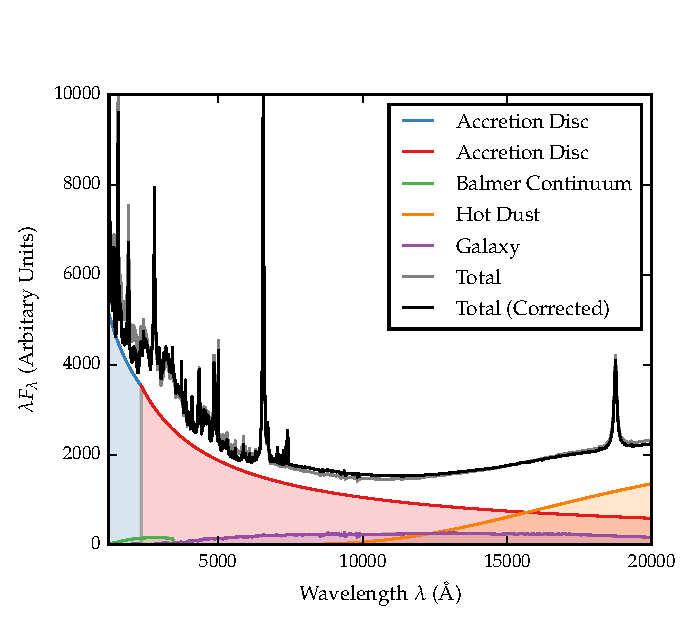
\includegraphics[width=\textwidth]{figures/chapter05/sed_model.pdf}
  \caption{Model spectrum at $z=1$, showing the contributions to the total flux from the blue power-law slope, red power-law slope, blackbody and host galaxy. The locations of the most prominent emission lines in the spectrum are also indicated. }
  \label{fig:modelsed}
\end{figure}

I have constructed a new SED model which reproduces the SEDs of AGNs from the rest-frame UV ($\sim 0.1 \mu$m) to the rest-frame near-IR ($\sim 3 \mu$m). 
In this section, I will describe how I have modelled the emission from the various components contributing to the emission in this spectral region. 
The model spectrum is shown in Figure \ref{fig:modelsed}, with each of the main components indicated. 

\subsection{Accretion Disk}

Thermal accretion disk emission in the 0.1 - 1 $\mu$m region is characterised by a broken power-law with three free parameters: a break-wavelength $\lambda_{\rm break}$, a blue power-law index $\alpha_{\rm blue}$ for wavelengths shorter than the break wavelength, and a red power-law index $\alpha_{\rm red}$ for wavelengths longer than the break wavelength.

\subsection{Balmer Continuum}







 # Add Balmer Continuum and blur to simulate effect of bulk-velocity
    # shifts comparable to those present in emission lines

    wbcnrm = parfile['quasar']['balmercont']['wbcnrm']
    wbedge = parfile['quasar']['balmercont']['wbedge']
    bcnrm = parfile['quasar']['balmercont']['bcnrm']
    tbc = parfile['quasar']['balmercont']['tbc']
    taube = parfile['quasar']['balmercont']['taube']
    vfwhm = parfile['quasar']['balmercont']['vfwhm']

gauss = Gaussian1DKernel(stddev=psigma)
    flux_bc = convolve(flux_bc, gauss)

    """
    inputs 
    
    wavlen = wavelength array 
    tbb = balmer continuum temperature
    fnorm = balmer continuum normalisation 
    taube = optical depth at balmer edge 
    wavbe = wavelength of balmer edge 
    wnorm = arbitary normalisation wavelength  
    relacc = related to computer precision - get rid of this 

    returns flux density per unit frequency 

    See https://arxiv.org/pdf/1311.6653 and Grandi (1982)

    See also Shen & Liu (2012)


\subsection{Hot Dust}

Thermal emission from hot dust, which dominates the \ac{SED} at wavelengths longer than $1\mu$m, is modelled using a simple blackbody

\begin{eqnarray}  
  F_\lambda =\frac{2 hc^2}{\lambda^5}\frac{1}{ e^{\frac{hc}{\lambda k_\mathrm{B}T}} - 1}, 
\end{eqnarray}

with two free parameters: the temperature $T_$ and normalisation relative to the power-law continuum. 

\subsection{Emission Lines}

We use an emission line template taken from \citet{maddox06}, who extend the composite of \citet{francis91} to include the H$\alpha$ (6560\AA) and Pa$\alpha$ (18750\AA) emission lines. 
A single free parameter, EL$_{\rm scale}$, scales the equivalent widths of all emission lines equally:

\begin{eqnarray}
  F_{\lambda} =  {\rm EL}_{\rm scale} \times \frac{F_{\lambda, \rm el}}{F_{\lambda, \rm cont}} \times F_{\lambda} 
\end{eqnarray} 

where $F_{\lambda, \rm el}$ is the line flux in the template, $F_{\lambda,\rm cont}$ is the continuum flux in the template, and $F_{\lambda}$ is the continuum flux in the model.  


scahal = params['scahal'].value

    # Normalise such that continuum flux at wavnrm equal to that
    # of the reference continuum at wavnrm
    inorm = wav2num(wavlen, wavnrm)
    flux = conval[inorm] * flux / flux[inorm]

    # Calculate Baldwin Effect Scaling for Halpha
    zbenrm = parfile['quasar']['el']['zbenrm']
    beslp = parfile['quasar']['el']['beslp']

    # Line added to stop enormous BE evolution at low z 
    zval = np.max([redshift, zbenrm]) 

    # I think this is the absolute magnitude of the SDSS sample as 
    # a function of redshift, which is not the same as how the 
    # absolute magnitude of a object of a given flux changes 
    # as a function of redshift 
    qsomag_itp = interp1d(qsomag[:, 0], qsomag[:, 1])

    # Absolute magnitude at redshift z minus
    # normalisation absolute magnitude
    vallum = qsomag_itp(zval) - qsomag_itp(zbenrm) 

    # Convert to luminosity 
    vallum = 10.0**(-0.4*vallum)

    scabe = vallum**(-beslp) 
     
    # ftmp = np.zeros_like(flux)
    # ftmp[:whmin] = linval[:whmin] * np.abs(elscal) * flux[:whmin] / conval[:whmin]
    # ftmp[whmax:] = linval[whmax:] * np.abs(elscal) * flux[whmax:] / conval[whmax:]

     
    flux[:whmin] = flux[:whmin] + linval[:whmin] * np.abs(elscal) * flux[:whmin] / conval[:whmin]
    flux[whmax:] = flux[whmax:] + linval[whmax:] * np.abs(elscal) * flux[whmax:] / conval[whmax:]

    # Scaling for Ha with Baldwin effect 
    scatmp = elscal * scahal / scabe
    # ftmp[whmin:whmax] = linval[whmin:whmax] * np.abs(scatmp) * flux[whmin:whmax] / conval[whmin:whmax] 
    flux[whmin:whmax] = flux[whmin:whmax] + \
                        linval[whmin:whmax] * np.abs(scatmp) * flux[whmin:whmax] / conval[whmin:whmax] 


\subsection{Host Galaxy}

Emission from the host galaxy must be accounted for, particularly in the region around the $1\mu$m inflection point in the quasar SED. 
We use a $z=0$ Sb template from \citet{mannucci01}, which does not evolve with redshift.
The template is scaled by a multiplicative factor $C$ and added to the \ac{AGN} \ac{SED}. 
We define a new parameter, $\eta$, the fractional contribution from the host galaxy to the total flux in the interval 4000 and 5000\AA:

\begin{eqnarray}
  \eta \equiv \frac{CF_{\rm Gal}}{F_{\rm AGN} + CF_{\rm Gal}},
\end{eqnarray}

where $F_{\rm Gal}$ and $F_{\rm AGN}$ are the flux of the galaxy and \ac{AGN} respectively. 
Rearranging for the scaling factor $C$ gives:

\begin{eqnarray}
  C = \frac{\eta}{1 - \eta} \frac{F_{\rm AGN}}{F_{\rm Gal}}.
\end{eqnarray}

The fractional contribution to the total emission coming from the host galaxy changes as a function of the \ac{AGN} luminosity and, in a flux-limited sample, the mean \ac{AGN} luminosity increases as the redshift increases. 
We parameterize the \ac{AGN} luminosity dependence of the host galaxy luminosity as a power-law:

\begin{eqnarray}
  \label{eq:lgal}
  \frac{L_{\rm Gal}}{L_{\rm AGN}} &=& L_{\rm AGN}^{\beta - 1} 
\end{eqnarray}

with slope $\beta=0.42$ \citep{maddox06}. 
The galaxy scaling factor $C$ becomes 

\begin{eqnarray}
  C &=& \frac{\eta}{1 - \eta} \frac{F_{\rm AGN}}{F_{\rm Gal}} \left[ \frac{ L_{\rm Gal}(z)} {L_{\rm AGN}(z)} \right] \left[ \frac{ L_{\rm Gal}(z_{\rm nrm})} {L_{\rm AGN}(z_{\rm nrm})} \right]^{-1} \\
  &=& \frac{\eta}{1 - \eta} \frac{F_{\rm AGN}}{F_{\rm Gal}} \left[ \frac{L_{\rm AGN(z)}} {L_{\rm AGN(z_{\rm nrm}})} \right]^{\beta -1}, 
\end{eqnarray}

where $z_{\rm nrm}$ is an arbitary redshift at which the fractional contribution from the host galaxy is by definition $\eta$. 
The redshift dependence of the mean \ac{AGN} luminosity for the SDSS quasar catalogue has been determined empirically, and is used to compute the term in the square brackets. 

\subsection{Dust Extinction}
\label{sec:sed-extinction} 

The selection criteria of the SDSS DR7Q catalogue are sensitive to quasars with moderate amounts of dust reddening \citep[possibly as high as E(B-V) $\sim$ 0.5;][]{richards03} at the redshift of the quasar, and so we included the effect of dust extinction in our model. 
We considered four types of extinction curve: the Large Magellanic Cloud (LMC), Small Magellanic Cloud (SMC), Milky-Way (MW) extinction curves from \citet{pei92} and an extinction curve appropriate for the quasar population which has been derived by Paul Hewett. 
To derive the quasar extinction curve, UKIDSS photometry was used to provide an E(B-V) estimate, via the magnitude displacement of each quasar from the locus of unreddened objects. 
At redshifts $2 < z < 3$ the reddening measure is made at rest-frame wavelengths 3500-7000\AA, where Galaxy, LMC and SMC extinction curves are very similar. 
The SDSS spectra of the same objects are then employed to generate an empirical extinction curve in the ultraviolet, down to 1200\AA. 
The resulting curve has no 2200\AA~ feature and rises rapidly with decreasing wavelength but is not as steep as the SMC curve. 
The extinctions curves give the colour excess $E(B-\lambda)$ relative to the colour excess $E(B-V)$ as a function of wavelength $\lambda$. 
The colour excess $E(B-V)$ is related to the extinction in the $V$ band, $A(V)$, via a parameter $R$, 

\begin{eqnarray}
  A(V) = R \times E(B -V )
\end{eqnarray}

where $R = 3.1$ in the MW and $R \simeq 3$ in the Magellanic Clouds. 
Hence the extinction at a wavelength lambda $A(\lambda)$ is 

\begin{eqnarray}
  A(\lambda) = E(B-V) \times \left[ \frac{E(\lambda-V)}{E(B-V)} + R \right] 
\end{eqnarray}

where the colour excess $E(B-V)$ is a free parameter in our model. 
The attenuation of the flux at a given wavelength is then:

\begin{eqnarray}
  F_\lambda = F_\lambda10^{-A(\lambda)/2.5}
\end{eqnarray}

in the rest frame of the quasar. 

\section{The `Standard' SED Model} 

\todoinline{
\begin{itemize}
    \item Given the same parameters, my model and Paul's look identical 
    \item I'm generating model colours using my model and Paul's best-fit parameters, and Paul's correction
    \item Do my model colours look the same as Paul's? (i.e. is there a bug in my code?)
    \item Can I generate the same median colours as Paul? (i.e. what sample is being used?)
    \item Can I do my own fit to the data?  
\end{itemize}  
}

We will begin by deriving a `standard' SED model by constraining a single set of parameters with a large sample of $0.2 < z < 4$ quasars encompassing a range of luminosities, accretion rates etc. 
The free parameters in our model are the blue power-law slope, the red power-law slope, the power-law break wavelength, the blackbody temperature, the blackbody normalisation, the emission line equivalent width scaling, and the fractional contribution from the host galaxy to the total flux. 
The reddening E(B-V) is fixed to zero, since a large fraction of SDSS quasars have very small amounts of dust reddening \citep{richards03}. 
For the host galaxy we use a Sb-type template derived by \citet{mannucci01}. 
With some choice of initial parameters, we generate a set of model observed spectra at redshifts from $z=0.25$ to $z=3.75$ in intervals of $\Delta z = 0.1$. 
We then transform our set of model spectra into a set of model $ugrizYJHKW1W2$ SEDs 

\begin{figure}
  \centering
  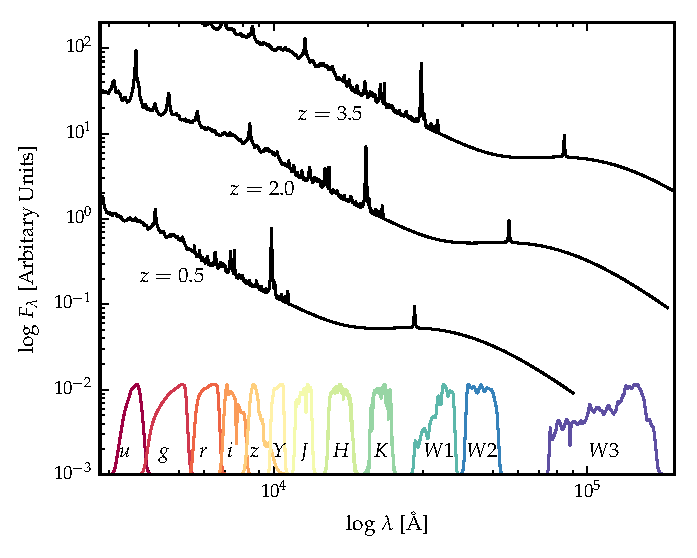
\includegraphics[width=\textwidth]{figures/chapter05/throughput.pdf}
  \caption{Model spectrum at three different redshifts (each arbitrarily scaled), and throughput functions for SDSS, UKIDSS and WISE band-passes.}
  \label{fig:filters}
\end{figure}

The throughput functions of the SDSS $ugriz$, UKIDSS $YJHK$ and WISE $W1W2W3$ band-passes are shown in Figure \ref{fig:filters}, along with our model AGN spectra at three different redshifts. 
The mean flux density in a band-pass P is given by 

\begin{eqnarray}
  \label{eq:flux}
  f_{\lambda}(P) & = & \frac{\int P(\lambda) f_\lambda(\lambda) \lambda d\lambda }{\int P(\lambda) \lambda d\lambda}
\end{eqnarray}

where $P(\lambda)$ is the dimensionless throughput function of the band-pass. 
The corresponding magnitude, $m_\lambda(P)$, is then 

\begin{eqnarray}
  m_\lambda(P) & = & -2.5{\rm log}(f_\lambda(P)) - m_0(P)
\end{eqnarray}

where $m_0(P)$ is the zero-point magnitude of band $P$. In the AB magnitude system, the zero-point flux per unit wavelength is 

\begin{eqnarray}
  \frac{f_\lambda(\lambda)}{{\rm erg}~{\rm cm}^{-2}~{\rm s}^{-1} {\rm\AA}^{-1}} = 0.1087 \left(\frac{\lambda}{\rm \AA}\right)^{-2} .
\end{eqnarray}

This is substituted into Equation \ref{eq:flux} to give a zero-point mean flux density which is then converted into a corresponding magnitude.  

The model SEDs are normalised such that the $i$ magnitude of each model SED is 18.0 mag. 
This gives us an array of model magnitudes as a function of redshift and band-pass. 
We generate an equivalent data array by dividing our quasar sample into redshift bins from $z=0.2$ to $z=3.8$ with bin width $\Delta z = 0.1$. 
We normalise the individual quasar SEDs such that the observed $i$ magnitude is equal to 18.0 mag, and then calculate a median SED in each redshift bin. 

To fit the model to the data we minimise the sum of the squares of the differences between the elements in the model magnitude array and the elements in the data magnitude array. 
The minimisation is done using the `nelder-mead' algorithm. 
Our SED model is valid only up to $\lambda \sim 3\mu$m in the quasar rest frame (the approximate wavelength of the peak in hot dust emission); beyond this additional contributions to the total flux from cooler dust will become significant. 
This prevents us from using the two highest wavelength WISE bands in the fit. 
We also exclude the SDSS $u$ and $g$ band-passes from the fit at $z > 2.7$ and $z > 3.7$ respectively, where absorption in the Lyman$\alpha$ forest becomes large. 

The best-fitting parameters from the fit are shown in Table \ref{tab:params}. 
\todo{Re-do fit}
The colours ($u - g$, $g - r$, etc.) of the median SED, the individual quasars, and the best-fitting model are plotted as a function of redshift in Figs.~\ref{fig:color_1} and \ref{fig:color_2}.  
Most of the large variations that can be seen in the median colours of the quasars as a function of redshift are due to strong emission lines being redshifted in to and out of the bandpasses of the band-passes being used. 

\begin{table}
  \centering
  \begin{tabular}{c c c}
    \hline 
    Parameter & Symbol & Value \\
    \hline 
    Blue power-law index & $\alpha_{\rm blue}$ & 0.58 \\
    Red power-law index & $\alpha_{\rm red}$ & -0.04 \\
    Power-law break & $\lambda_{\rm break}$ & 2945 \\
    Blackbody temperature & $T_{\rm BB}$ & 1216 K \\
    Blackbody normalisation & $C_{\rm BB}$ & 0.22 \\
    Emission line scaling & $C_{\rm EL}$  & 0.63 \\
    Galaxy fraction & $\eta$ & 0.29 \\
    E(B-V) & E(B-V) & 0.00 \\
    \hline
  \end{tabular}
  \caption{Best-fitting parameters.}
  \label{tab:params}
\end{table}

\begin{figure}
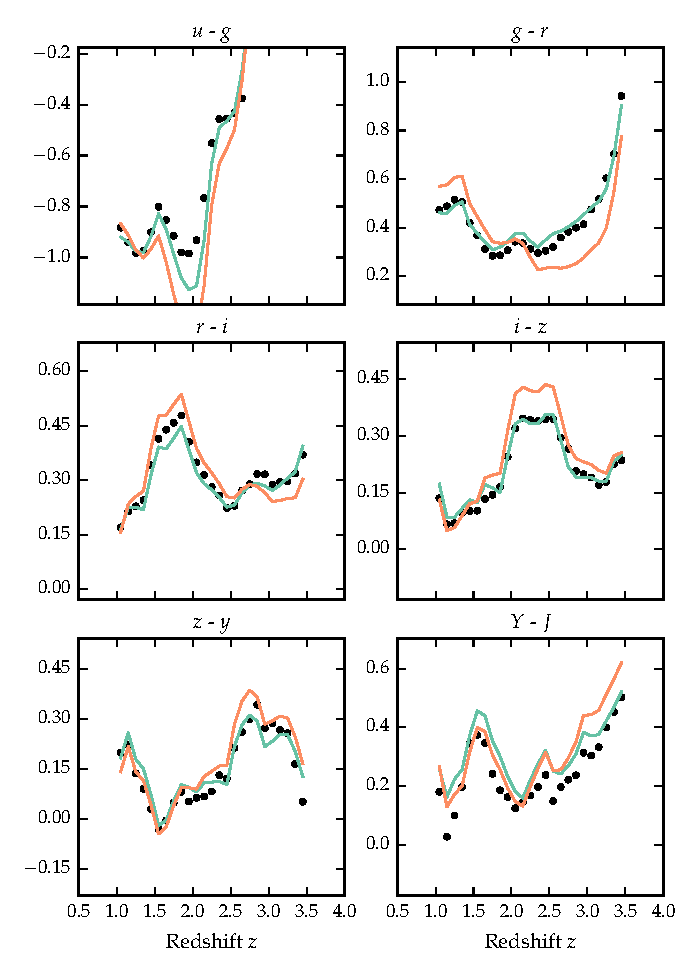
\includegraphics[width=\textwidth]{figures/chapter05/sed_color_plot_1.pdf}
\caption{Colours of median SED and best-fitting model, with and without correction}
  \label{fig:color_1}
\end{figure} 


\begin{figure}
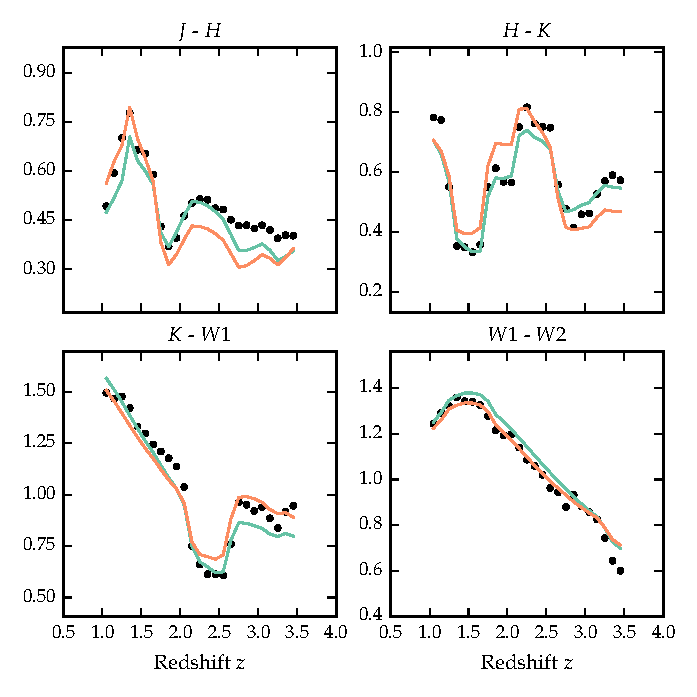
\includegraphics[width=\textwidth]{figures/chapter05/sed_color_plot_2.pdf}
\caption{Colours of median SED ({\it black circles}), individual objects ({\it grey points}), best-fitting  model ({\it black line}) as a function of redshift.}
  \label{fig:color_2}
\end{figure} 

\section{Discussion of Fit}

\begin{figure}
  \centering
  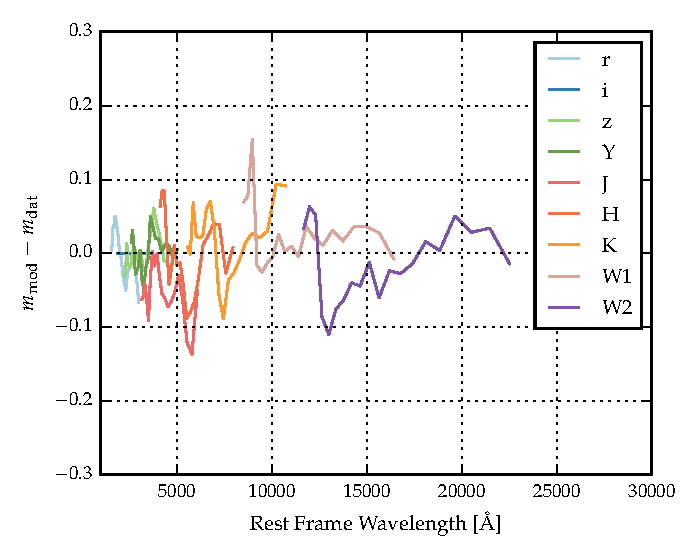
\includegraphics[width=\textwidth]{figures/chapter05/model_residuals.pdf}
  \caption{Residuals from fit as a function of rest-frame wavelength. \todoinline{Show before and after correction.}}
  \label{fig:residuals}
\end{figure}

In Figure \ref{fig:residuals} we show the difference between the magnitudes from the best-fitting model and the median magnitudes from the sample. 
We have transformed the effective wavelengths of the band-passes to the rest frame of the quasars in each redshift bin, to give to the residuals as a function of rest-frame wavelength. 
We represent the residuals measured in each band-pass using a different coloured line. 
Differences between residuals from different band-passes at the same rest-frame wavelength could indicate redshift evolution of the typical quasar SED. 

The residuals indicate that over a large redshift range the model does a fairly good at reproducing the median observed colours of the sample. 
Most discrepancies are at the $<0.1$ mag level. 
It is remarkable that a single model is so effective; the properties of a typical quasar to not change significantly over a wide range of redshifts and luminosities. 
On the other hand, for the individual objects there is a significant scatter about the mean. 
In general, our goal is to use this intrinsic spread in SED properties in order to understand the diversity in physical quasar properties. 

\subsection{Flux Correction}

The most noticeable feature in Figure \ref{fig:residuals} is a bump around 1$\mu$m, where the model underestimates the flux of the population by $\sim 0.1$ mag. 
If the model is a poor fit to the data, it can produce strong redshift-dependent systematics. 
A blackbody component with a higher temperature would contribute more flux in this region, which could potentially lead to redshift-dependent systemetatic errors. 
To avoid this we derived a correction to our model which accounted for the $1 \mu$m flux discrepency. 
\todo{Describe Paul's empirical correction.}

\section{Hot Dust}

Including a black-body with T$\sim$1250K, a simple parametric model matches the ugrizYJHKW1W2 (SDSS+UKIDSS+WISE) median colours of luminous quasars at redshifts $0.2 < z < 0.4$ extraordinarily well \todo{Don't use words like extraordinary}. 
The spread in the KW1W2 colours (Figure~\ref{fig:w1w2colorsratio}), probing the rest-frame $\sim$1-2 micron region, is significant and strongly suggests presence of real variation in the "hot dust" temperature and luminosity among the quasars. 

\subsection{Parameterising the hot dust emission}

We characterise the hot dust properties of our sample in terms of the temperature and luminosity of a blackbody.  
We choose to parameterise the luminosity in terms of the NIR to UV luminosity ratio (which is proportional to the covering factor of hot dust ($L_{NIR}/L_{Bol}$) used in other studies \citep{roseboom13}. 
The UV and NIR luminosity are calculated between 2000 and 9000\AA and 1 and 3 $\mu$m respectively.

In Figure~\ref{fig:ratio_tbb_density} we see that the two parameters are clearly correlated. 
For a lower temperature black-body the NIR to UV luminosity ratio is larger. 
Such a correlation is to be expected: as the black-body temperature is lowered, the peak shifts to longer-wavelengths (following Wien's displacement law). 
Because of this degeneracy we need to be very careful to seperate out real trends of $R_{NIR/UV}$ with other quasar properties from indirect trends resulting from a mutual dependence on $T_{BB}$.  

\begin{figure}
  \centering
  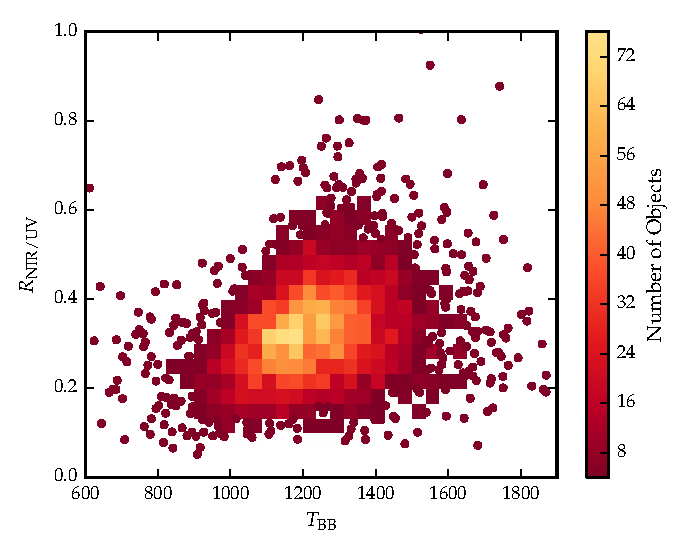
\includegraphics[width=\textwidth]{figures/chapter05/ratio_tbb_density.pdf}
  \caption{Ratio of NIR to UV luminosity ($R_{NIR/UV}$) against temperature ($T_{BB}$) for low-$z$ sample. The density of points is shown in more dense regions of the space, and individual objects in less dense regions. }
  \label{fig:ratio_tbb_density}
\end{figure}

Some previous studies \citep[e.g.][]{wang13,zhang14} have instead paramterised the near-IR emission using a power-law.
Emission in near-ir generally characterised either by a power-law ($\propto \lambda^{\beta_{\rm NIR}}$), with $\beta \simeq 0.5$ \citep[e.g.][]{richards06, zhang14}. 
We tested this parameterisation, and evaluated it's effectiveness relative to using a black-body. 
The power-law is normalised at 9000A, where its flux is set equal to the flux of the UV/optical model. 
The NIR power-law slope is fit between $\sim$1 and 2.4$\mu$m (with the exact wavelength region being fit depending on the redshift of the quasar). 
We found large residuals in the best-fitting model which varied systematically as a function of $\lambda_{eff}/(1+z)$.  
This suggests that the power-law model is a poor fit to the shape of the near-IR emission. 
One needs to take care in looking at trends with luminosity given the observed-frame passband information on the rest-frame SED can produce some strong systematics with redshift, particularly if the SED-model is not a good fit to the actual SED. 
A similar conclusion was reached by Gallagher et al.

\subsection{Sample}

Our goal is to determine the temperature and abundance of the hot dust component in individual quasars.  
These properties will be measured by fitting a model to the SDSS-UKIDSS-WISE photometry. 
Constraing a T$\sim$1200K blackbody component in the SED model requires photometric data covering $\sim$1-3$\mu$m in the rest-frame of the quasar. 

The observed-frame wavelength coverage of the available passbands limits the redshift range of the quasars which can be used. 
One does need to take care in looking at trends with luminosity given the observed-frame passband information on the rest-frame SED can produce some strong systematics with redshift, particularly if the SED-model is not a good fit to the actual SED. 
We consider only quasars at redshifts $z>1$ where the relative host galaxy contribution to the SED is negligible. 
At redshifts $1 \lesssim z \lesssim 1.5$ the available ugrizYJHKW1W2 photometry provides good coverage of the rest-frame SED up to $\sim$2$\mu$m.
At $z\sim1.5$ the W2 passband is shifted to $\sim$1.8$\mu$m; at higher redshifts the wavelength coverage of the W2 band becomes much less than the peak wavelength of a T$\sim$1200K blackbody and experiments showed that such a component can not be adequatly constrained by the available photometry. 
Quasars in the redshift interval $1.5 < z < 2$ are therefore excluded from our sample. 

For the quasars at $z \sim 1$ the WISE W3 band is probing rest-frame wavelengths of $\sim5-6\mu$m. 
This region of the SED is dominated by emission from cooler, more distant dust, which is not accounted for in our model.
However, at redshifts $z \gtrsim 2$ the WISE W3 passband probes sufficiently short wavelengths to be useful in constraining the shape of the hot blackbody component. 
Therefore for quasars at redshifts $z > 2$ we again have sufficient constraints from the ugrizYJHKW1W2W3 photometry to determine the temperature and normalisation of the blackbody component. 
There are few objects in our sample with redshifts $z > 2.7$, and so we set this as an upper limit on the redshift of our sample. 
Because of these constraints, our sample is divided in to two parts: one at low redshifts ($1 < z < 1.5$) and the other at higher redshifts ($2 < z < 2.7$). 

We include only quasars with observed magnitudes brighter than 19.1 in the $i$ band-pass, i.e. the quasars selected by the main SDSS quasar selection algorithm (70,214 quasars). 
Cross-matching (with a 2$''$ radius and picking only the nearest neighbour) the SDSS DR7Q catalogue with the ULAS catalogue, which covers only $\sim 38$\% of the SDSS foot-print, resulted in 37,886 matches. 
Of these 36,628 have been detected in one or more of the WISE band-passes. 
We exclude quasars flagged as broad-absorption line quasars from the sample (leaving 35,272 quasars).
We impose a lower-limit signal-to-noise ratio (S/N) $>$ 5 magnitudes in the $K$, $W1$ and $W2$ band-passes for the low-$z$ sample and S/N > 5 in the $W1$, $W2$, and $W3$ band-passes for the high-$z$ sample to ensure reliable photometry. 
This gives us 5,910 quasars in our low-$z$ sample and 1,989 quasars in our high-$z$ sample. 

We will hold most parameters fixed, and vary only those we are interested in, i.e. the blackbody parameters which parameterise the NIR emission. 
Therefore we need to define a sub-sample of objects which we know are well fit by our standard SED model in the UV/optical region. 
This means excluding objects with extreme emission line equivalent widths or significant dust extinction.
We use the $i-K$ colours of the quasars as a measure of the overall colour of the quasars as it provides the longest baseline in wavelength without being affected by absorption in the Ly$\alpha$ forest at high redshifts. 
A significant amount of this reddening can be attributed to intrinsics variations in the UV power-law slopes of the indidual quasars, which is why we allow a negative reddening. However, there is a clear `red tail' to the colour distribution which can be explained by dust reddending at the redshift of the quasar.
We discarded from our sample quasars with $i - K$ colors redder than our standard model with dust reddening E(B-V) = 0.075 and bluer than E(B-V) = -0.075 (Figure~\ref{fig:ikzplot}). 
Following this cut we are left with 4,615 quasars in our low-$z$ sample and 1,692 quasars in our high-$z$ sample. 

\begin{figure}
  \centering
  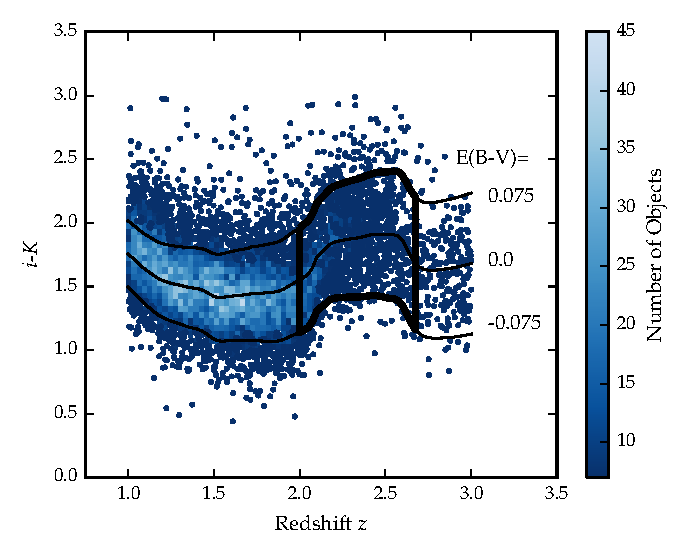
\includegraphics[width=\columnwidth]{figures/chapter05/ik_versus_z_low_ext.pdf}
  \caption{$i-K$ colours of non-BALQSO DR7Q quasars with $i>19.1$ as a function of redshift. The lines show the colours of our model with varying amounts of dust extinction. Quasars with extinction $|E(B-V)|>0.075$ are excluded.}
  \label{fig:ikzplot}
\end{figure}

\subsection{Diversity in hot dust properties}

In Figure~\ref{fig:w1w2colorsratio} we plot the $W1 - W2$ colors of the sample as a function of redshift at z < 3. 
In this redshift range the $W1$ and $W2$ band-passes are probing the 1.2 - 2.8$\mu$m and 1.6 - 3.8 $\mu$ region of the rest frame SED respectively. 
For reference, the peak wavelength is at 2.4$\mu$m for a black-body radiating at 1200K (close to the sublimation temperature of dust grains). 
At any given redshift we see a $\sim 0.5$ mag dispersion in the $W1-W2$ colors. 

On the same axes in the Figure we have plotted the $W1 - W2$ colors derived from our SED model with a fixed blackbody temperature (1216K) and a ratio of NIR to UV luminosity ranging from 0.0 to 1.0, with the other model parameters held constant. 
We conclude that even with the sample restricted to be fairly uniform in its UV/optical properties, we still get an interesting spread in W1-W2 colors, which we can use to learn about the diversity of NIR properties in our sample. 
In the rest of this chapter we will characterise the hot dust properties of our sample, and test its relation to quasar properties such as luminosity, black-hole mass and normalised accretion rate, and outflow-properties. 

\begin{figure}
\centering
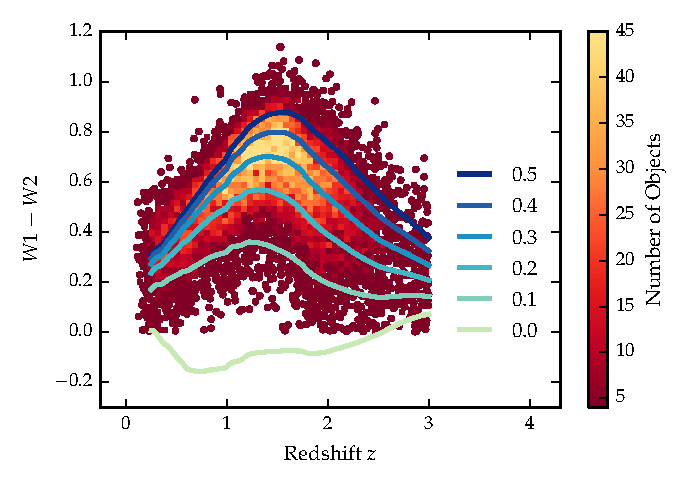
\includegraphics[width=\columnwidth]{figures/chapter05/w1w2_versus_redshift_ratio.pdf}
\caption{$W1 - W2$ colours of sample as a function of redshift. Above a certain density threshold points are represented by a density plot. On top we plot the colours of our standard SED model, with a fixed temperature and a varying NIR (1 - 3 $\mu$m) to UV ratio.}
  \label{fig:w1w2colorsratio}
\end{figure}

In Figure~\ref{fig:ratio_tbb_density} we show that there is quite a range of temperature and normalisation present in our sample. 
However, we need to check how much of this is due simply to uncertainties in the fits stemming from uncertainties in the photometry. 
In order to achieve this we took our standard SED model with a single temperature and normalisation black-body component, and generated 200 mock SEDs with a brightness distribution similar to that of our real sample. 
We estimated the mean uncertainty of the magnitudes in the K, W1, and W2 band-passes as a function of apparent brightness. 
We then sampled the K, W1, and W2 magnitudes from Gaussian distributions, with a mean equal to the magnitude of the model SED, and the width equal to the mean uncertainty at the appropriate brightness. 
Finally, we fit these mock SEDs using our standard fitting procedure. 
The results are shown in the Figure below, on top of the results from our real sample (shown as grey contours). 
We can see that uncertainty in the photometry introduces a significant scatter to the temperature, but that this scatter is less than the intrinsic scatter in the data. 
This demonstrates that there is a real distribution of hot dust temperatures and luminosities in our sample. 

\begin{figure}
  \centering
  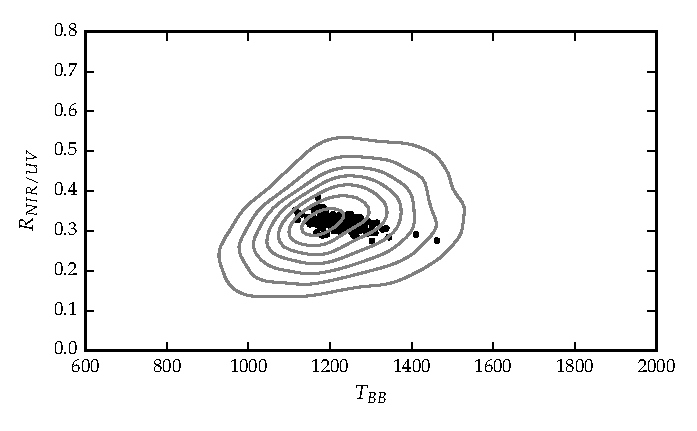
\includegraphics[width=\textwidth]{figures/chapter05/ratio_tbb_contours.pdf}
  \caption{Ratio of NIR to UV luminosity ($R_{NIR/UV}$) against temperature ($T_{BB}$). The grey contours show equally-spaced lines of constant probability density generated using a Gaussian kernal-density estimator on our data sample. The black points are for our mock data.}
  \label{fig:ratio_tbb_contours}
\end{figure}

\section{Fitting procedure}

We will fit a model to the individual quasar SEDs, allowing the temperature and normalisation of the black body component to vary. 
The model spectrum is redshifted to the redshift of the quasar being fit and is then multiplied by the $ugrizYJHMW1W2W3$ throughput functions and normalised appropriately to give AB magnitudes. 
To fit the model to the data we minimise the sum of the squares of the differences between the elements in the model magnitude array and the elements in the data magnitude array. 
To avoid significant absorption in the Lyman-$\alpha$ forest at high-$z$, we restrict our fitting to wavelengths greater than 2000A; when the effective wavelength of a band-pass falls below this limit the band-pass is excluded from the fit. 
The minimisation is done using the 'nelder-mead' method, as implemented in the ${\tt minimize}$ function from the Python module ${\tt scipy}$. 
\todo{2000A is quite large given the Lyman-alpha forest impacts from 1216A.}

\section{Results}

\subsection{Correlations with quasar properties}

\begin{figure}
  \centering
  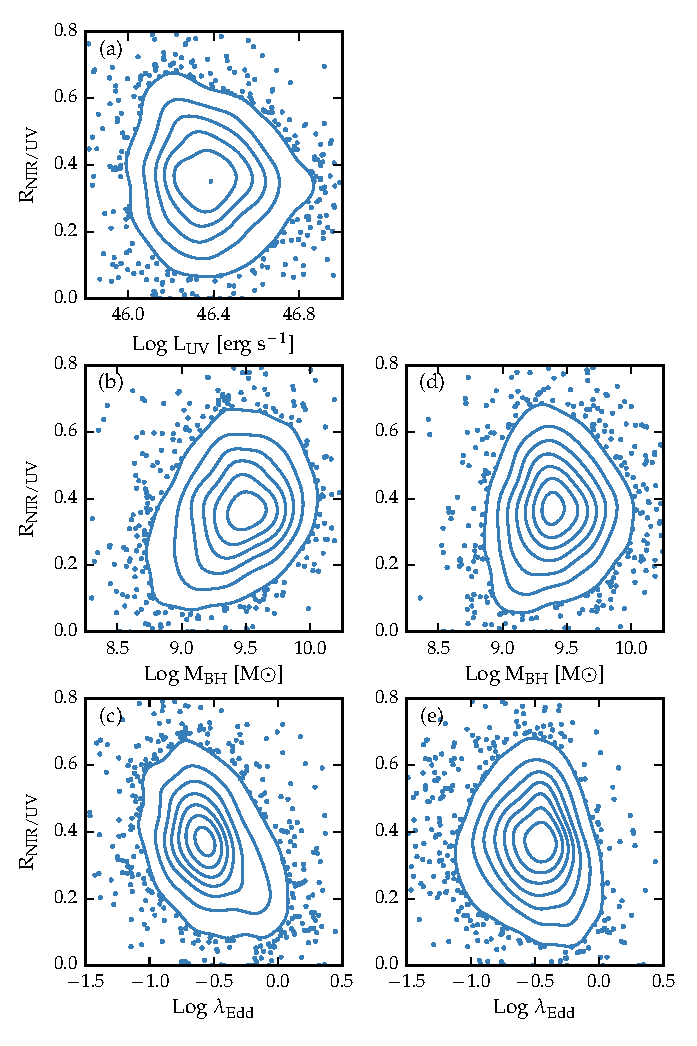
\includegraphics[width=\textwidth]{figures/chapter05/correlations_contour.pdf}
  \caption{Best-fit black-body temperature against UV luminosity (left), black-hole mass (center) and Eddington ratio (right) for $1 < z < 1.5$ sample (black) and $2 < z < 2.7$ sample (black). In region of high-density we represent the density with contours generated using a Gaussian kernel density estimation. \todoinline{Needs re-making with new BH masses.}}
  \label{fig:correlations_contour}
\end{figure}

We now look for correlations between the properties of the black-bodies we have fitted to the hot dust emission and other properties of the quasar such as redshift, black-hole mass, and normalised accretion rate (Eddington ratio). 
\todo{Calculate new BH masses and redo this section.}

% There is a clear anti-correlation between the UV luminosity and the best-fit black-body temperature. 
% We calculated a Spearman rank-order correlation coefficient -0.33. 
% \todo{Do we believe this trend is real?}
% \todo{This is just for low-z sample.}
% The black-hole masses are virial estimates calculated by Shen et al. 2011 using the MgII emission line in the SDSS spectra. 
% The Eddington ratios (bolometric luminosity normalised by Eddington luminosity) are also calculated by Shen et al. 2011 using bolometric corrections in Richards et al. (2006a) using 3000\AA monochromatic luminosities. 
% There are no significant correlations between $T_BB$ and $R_{NIR/UV}$ and the UV luminosity, black-hole mass or Eddington ratio. 

% The dynamic range in luminosity is very limited. 
% I will combine the low and high $z$ samples. 
% As first step see if there is a difference in the median $R_{NIR/UV}$ for low/high luminosity samples. 

% At low-$z$  we get a much larger range in black-body temperatures from our fits. 
% We discussed how the W3 S/N > 5 cut might be be biasing the high-z sample if the subset being removed had properties distinct from the remainder of the sample. 
% The W3 S/N > 5 cut removes about 25\% of the sample. 

% We observe a postive correlation between the black-hole mass and the NIR to UV luminosity ratio which is quite different from what we observed in our low-$z$ sample. 
% We believe that this is just a manifestation of the fact that at high redshift the black-hole masses are derived from CIV. 
% We will show below how the FWHM of CIV has a positive correlation with the hot dust abundance, and large CIV FWHM leads to larger black hole mass estimates. 
% This explains the apparent correlation between the IR/UV ratio and the black hole mass. 
% Eddington ratio measures the luminosity relative to the Eddington luminosity. 
% Higher blackhole mass estimates will lead to lower Eddington ratios, which is why the Eddington ratio appears to decrease with increasing IR/UV ratio. 
% For the sources in our low-$z$ sample the black-hole mass is measured using the broad MgII emission line. 
% As we will show below, the properties of the MgII emission line have no dependence on the hot dust properties. 

\subsection{Spectral properties}

In the dusty wind model - first proposed by \citet{konigl94} and later developed by, amonst others, \citet{everett05}, \citet{elitzur06}, \citet{keating12} - the `torus' is the dusty part of a magneto-hydrodynamic wind beyond the dust sublimation radius. 
The MHD wind is roughly polar, and so the hot dust forms a vertical `wall' around the accretion disk.  
UV photons from the accretion disk accelerate the wind via radiation line driving. 
That flattens the geometry of the wind and exposes more surface area that is viewable on a relatively face-on line of sight.  
The radiation pressure is increased at higher luminosities and/or accretion rates.
This can flatten the geometry of the wind, thereby increasing the range of angles for which the inner edge of the dusty wind - where dust is at it's sublimation temperature - can be observed. 
A direct prediction is therefore that the in a quasars with high accretion rates and strong outflows, the emission from hot dust should be enhanced. 

\subsubsection{Low-$z$}

\begin{figure}
  \centering
  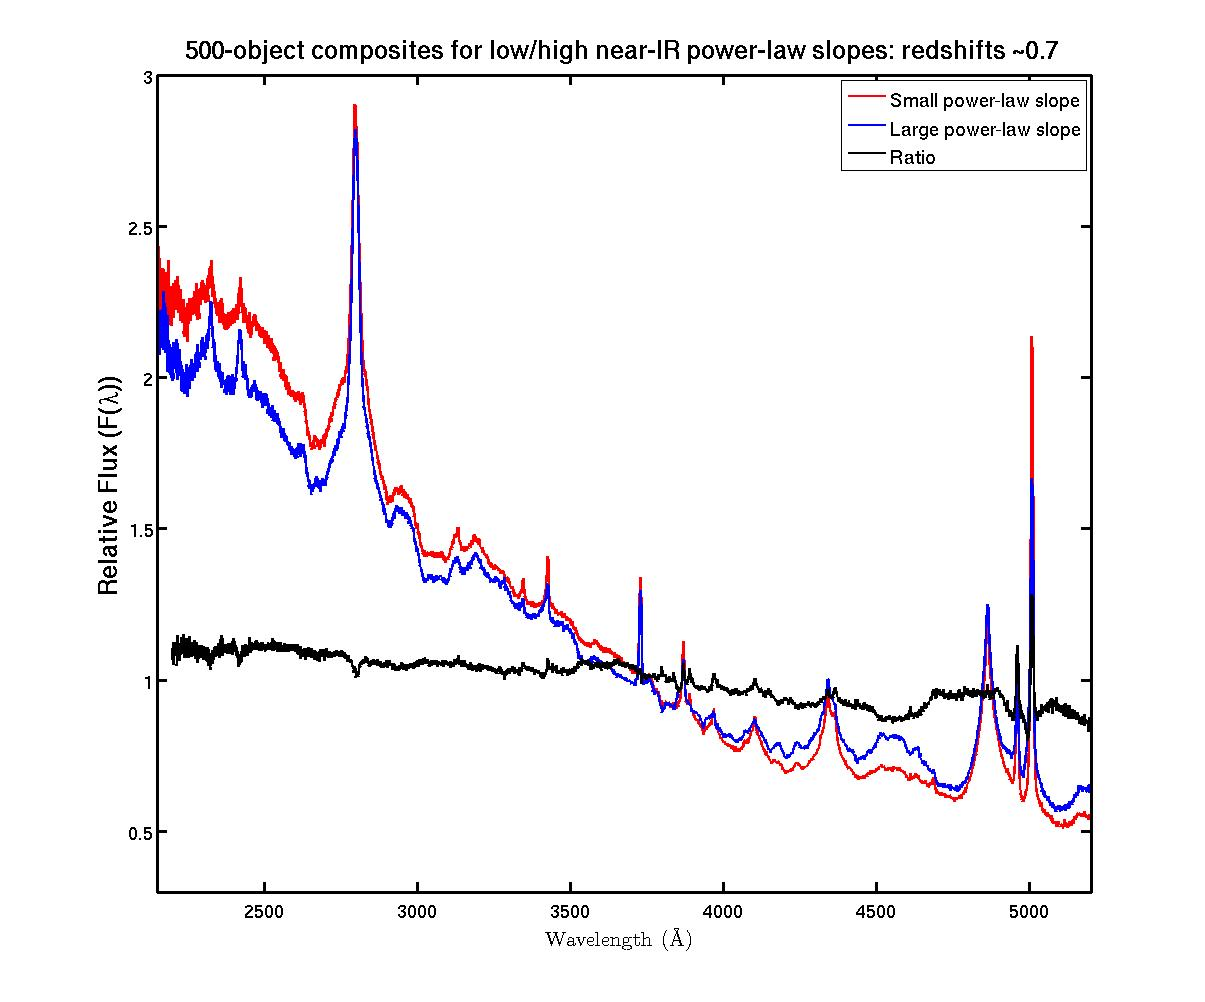
\includegraphics[width=\textwidth]{figures/chapter05/z07_pls_comps.jpg}
  \caption{Composite SDSS spectra for objects at $z\sim0.7$. We have divided sample into objects with objects best-fit by small (red line) and large (red line) values of $\beta$. \todoinline{Change this to select by $R_{NIR/UV}$ / $T_{BB}$. Label prominent emission lines.}}
  \label{fig:pls_comp}
\end{figure}

The $z < 0.8$ SDSS spectrum composite comparison for the small and large $\beta_{NIR}$ sub-samples is a very direct illustration of the \citet{boroson92} Eigenvector 1 describing the spectral variation in the optical spectra of quasars; as \ion{Fe}{II} EW increases the [\ion{O}{III}] EW decreases. 
Hot dust emission increases with \ion{Fe}{II} EW \citep{shen14}. 
We also note that the amount of hot dust correlates with the \ion{Si}{III}/\ion{C}{III}] emission ratios. 
The \ion{Si}{III}/\ion{C}{III}] ratio is generally considered to be a good indicator of density and is one of the primary EV1 correlates. 
The relative flux ratio of \ion{Si}{III} to \ion{C}{III}] increases when \ion{C}{IV} is more blue-shifted \citep{richards11}. 
The \ion{Mg}{II} emission line has exactly the same profile/shape for the two samples (apparent changes in \ion{Mg}{II} seen in Fig.~\ref{fig:pls_comp} are the result of changes in \ion{Fe}{II} at wavelengths just shortward of the line). 
Finally, we note that objects with more hot dust are slightly redder.

\subsubsection{High-$z$}

In Fig.~\ref{fig:civ_hot_dust} we show how the ratio of NIR to UV luminosity depends on the blueshift and rest-frame equivalent width of the \ion{C}{IV} line.
\ion{C}{IV} blueshifts are calclulated as in Section XX. 
We see that the NIR to UV luminosity ratio is strongly correlated with the blue-shift of the \ion{C}{IV} emission line. 
A similar trend was noted by \citet{wang13}. 
Interestingly, we note strong similarities to the object subsets selected according to their \ion{C}{IV}-emission properties in \citet{richards11} (see Figures 11 \& 12).  
We note that the correlation between the hot dust and the \ion{C}{IV} emission properties will lead to apparent correlations between the host dust and the BH mass. 
\todo{Need to re-do this and understand why beta-related trend is apparently stronger than with the blackbody parameters.}
 
\begin{figure}
\centering
  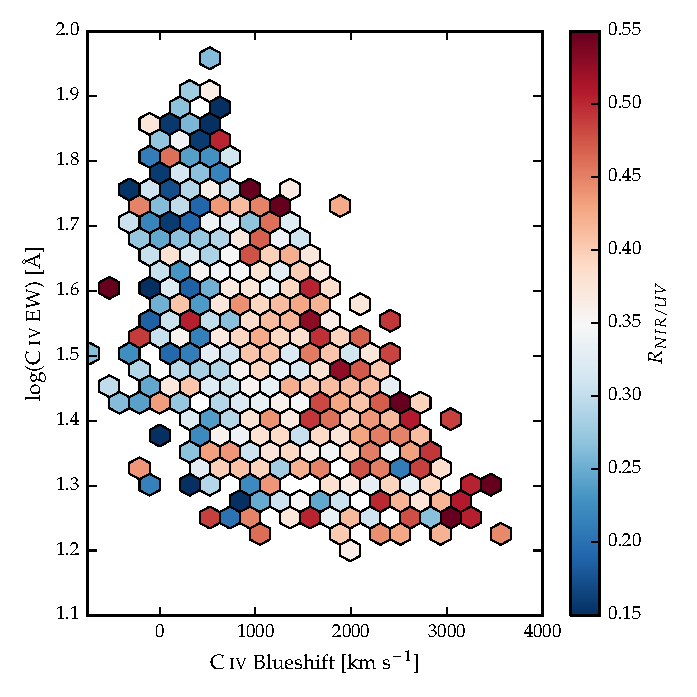
\includegraphics[width=\columnwidth]{figures/chapter05/hot_dust_ratio.pdf}
  \caption{Rest-frame equivalent width and blueshift of the \ion{C}{IV} line for 7,115 SDSS DR7 quasars. The colours of the hexagons denote the median hot dust (T$\simeq$1200\,K) abundance for all quasars at a given equivalent width and blueshift. Quasars with the most extreme outflow signatures are predominantly hot-dust rich. Only bins containing a minimum of two objects are plotted.}
  \label{fig:civ_hot_dust}
\end{figure}

\begin{figure}
\centering
  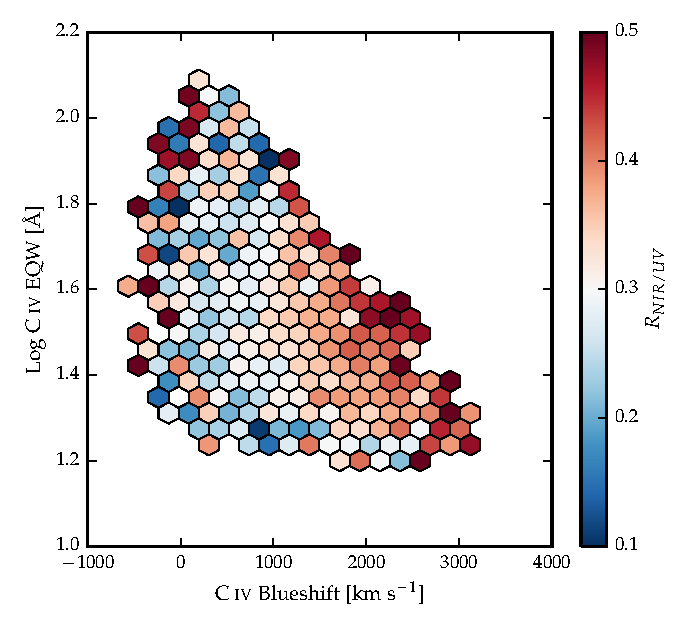
\includegraphics[width=\columnwidth]{figures/chapter05/hot_dust_beta.pdf}
\caption{Rest-frame equivalent width and blueshift of the \ion{C}{IV} line for 7,115 SDSS DR7 quasars. The colours of the hexagons denote the median hot dust (T$\simeq$1200\,K) abundance for all quasars at a given equivalent width and blueshift. Quasars with the most extreme outflow signatures are predominantly hot-dust rich. Only bins containing a minimum of two objects are plotted. \todoinline{Change hot dust abundance.}}
  \label{fig:hot_dust_beta}
\end{figure}

\begin{figure}
\centering
  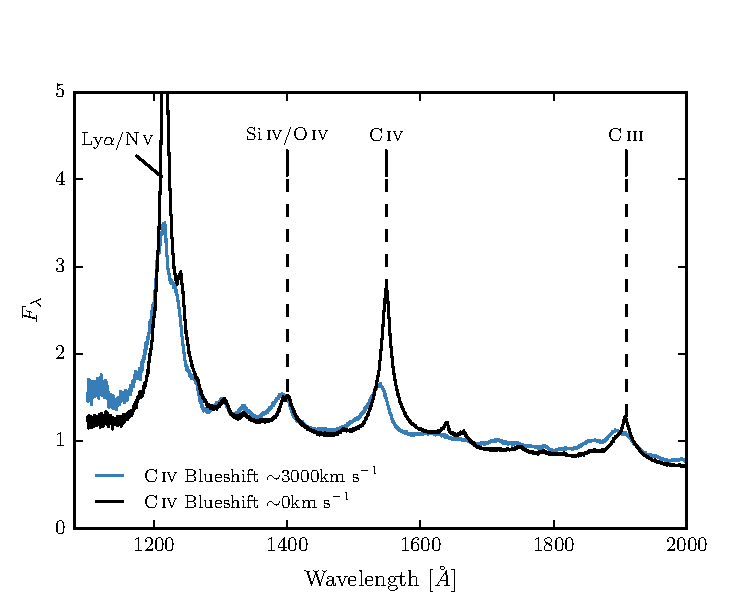
\includegraphics[width=\columnwidth]{figures/chapter05/blueshift_composite.pdf}
\caption{}
  \label{fig:blueshift_composite}
\end{figure}

\subsection{BALs and radio-loud/radio-quiet}

In the spectra of about 20\% of all quasars we observe broad (> 2000km/s) blue-shifted absorption troughs which are associated with quasar-driven out-flowing gas. 
BAL quasars in general have redder UV continua than non-BAL quasars, which is interpreted as the result of dust extinction. 
BAL quasars, on average, also have higher Eddington ratios and luminosities than non-BAL quasars.

We defined a sample of BAL quasars using the same method we used to define our sample of non-BAL quasars. 
\todo{Need to justify our use of model which has been optimised to fit colours of non-BAL quasars, when we know that BALs are typically redder.} 
At $1 < z < 1.5$ there are very few BAL quasars in our sample. 
In the $2 < z < 2.7$ redshift region we have 394 HiBAL quasars (the wavelength coverage of the SDSS spectra are not sensitive to LoBALs at these redshifts). 
\todo{What catalogue did we use to define quasar sample?} 
Since BAL quasars are expected to suffer more from extinction due to dust, we have allowed E(B-V) to vary for the BAL quasar sample. 

We find that the black-body temperature distributions are consistent (median $T_{BB}$ for both samples = 1180K), but the ratio of NIR to UV emission is higher in BALs ($R_{NIR/UV}$ = 0.92 and 0.83 for BAL and non-BAL quasar sample respectively). 
This is qualatatively consistent with the results of \citet{zhang14}. 

It is well known that the blueshift of the \ion{C}{IV} emission line in radio-quiet AGNs is, on average, stronger than in radio-loud AGNs (Marziani et al. 1996; Sulentic et al. 2000a; Richards et al. 2002, 2011). 
Statistically at least, the "radio-loud" objects are thought to have high black-hole masses and there is some form of radio-mode feedback (jet related) which is very different from the much more common (almost certainly wider opening-angle) outflow objects with large CIV-blueshifts.

So we find BALs have more hot dust, radio-loud have less. 
This is perfectly consistent with what we know about the positions of radio-loud objects and BALs in the \ion{C}{IV} parameter space distribution \citep{richards11}. 

\section{Other works}

\citet{roseboom13} studied a similar sample of luminous type 1 quasars. 
They, like us, modelled the NIR emission using a black-body and modelled the emission at longer wavelengths using a clumpy torus model. 
They find that while $L_{1-5\mu m}$/$L_{IR}$ appears relatively insensitive to $L_{bol}$ and $L_{IR}$, a strong correlation appears between $L_{1-5\mu m}$/$L_{IR}$ and $L_{IR}/L_{bol}$ (i.e. the dust covering factor). 
As the covering factor decreases, the maximum inclination at which a type 1 quasar would be seen increases. 
An increase in the inclination will mean direct sight lines to more of the inner wall of obscuring material closest to the accretion disc.

\citet{mor11} also looked at the hot dust properties of a sample of $0.75 < z < 2$ quasars, with photometry from SDSS and WISE. 
They modelled the NIR emission with hot clouds of pure graphite dust. 
They reported an anti-correlation between the covering factor of hot dust clouds and the quasar bolometric luminosity. 
Like us, they neglect cooler dust components which will dominate the SED at longer wavelengths. 
As we have discovered (see Figure residual plot), the missing flux decreases with redshift because we observe shorter rest-frame wavelengths when the observed spectrum is redshifted to a greater degree. 
This will induce an anti-correlation between the luminosity of the hot dust component and the luminosity of the quasar (which is correlated with redshift). 
At z=0.75, the W3 band-pass (the longest in their fits) is sensitive to flux from 6.9$\mu$m; at this wavelength we expect the contribution from cooler dust to dominate over the hot dust. 
It is possible that this effect could explain the tension with our own result that $R_{NIR/UV}$ does not depend on the quasar luminosity in our low-$z$ sample. 

\citet{shen14} quantify the relative torus emission using the $r-W1$ colour for a sample of $0.4 < z < 0.8$ SDSS quasars. 
At these redshifts W1 is observing between 1.9 and 2.4 microns in the rest-frame of the quasar, which suggets that they are sensitive to the same component of hot dust which we are investigating. 
They observe a mild trend of decreasing relative torus emission as the quasar luminosity increases. 
We note that their use of the r-W1 at much higher redshifts may be problematic, as the W1 flux will be increasingly dominated by direct emission from the accretion disc. 

\citet{gallagher07} undertook a similar investigation for a much smaller sample of 234 radio-quiet quasars.


\subsection{Eddington ratio}

Wang et al., Zhang et al., and Mor \& Trakhtenbrot find no significant dependence of the amount of hot dust on the Eddington ratio. 
Is this because the Eddington ratio is wrong or because it's more complicated? (can high accretion objects with no evidence for strong outflows.)

Shen \& Ho find that torus emission is enhanced in quasars with larger $R_{FeII}$. 
They show how EW(OIII) and other high-ionisation lines (and to a lesser extent low-ionisation lines like MgII) anti correlate with $R_{FeII}$. 
The enhancement of torus emission relative to accretion disc emission at the high-RFeII end of EV1 may be caused by more efficient disc winds that facilitate the formation of a dusty torus. 
From our $z\sim0.8$ composite SDSS spectra, we observed that objects with large NIR to UV luminosity ratios on average have stronger FeII emission. 

\section{Further work}

What more is needed to test model(s)?  